\section*{Problem Sheet 3:}
\label{sec:ps3}
\newcounter{psThreeQuestions}
\setcounter{psThreeQuestions}{0}
\renewcommand{\NewQuestion}[1]{\stepcounter{psThreeQuestions}\subsection*{Exercise \arabic{psThreeQuestions}: #1}}

\NewQuestion{Direct CP violation (exam style)}
\begin{enumerate}
\item Draw the tree level Feynman diagram for $B^0\to K^+\pi^-$
and $\bar{B}^0\to K^-\pi^+$ carefully labelling the CKM elements associated at each vertex
\item Are there any CKM phases associated with these diagrams and if so what are they?
\item CP violation requires the interference of two diagrams with different phases, such that this phase difference appears in the expression of the decay rates. Consider the loop-level Feynman diagram below. Explain why the diagram with the top quark running around the loop dominates. What is its overall CKM phase?
\begin{center}
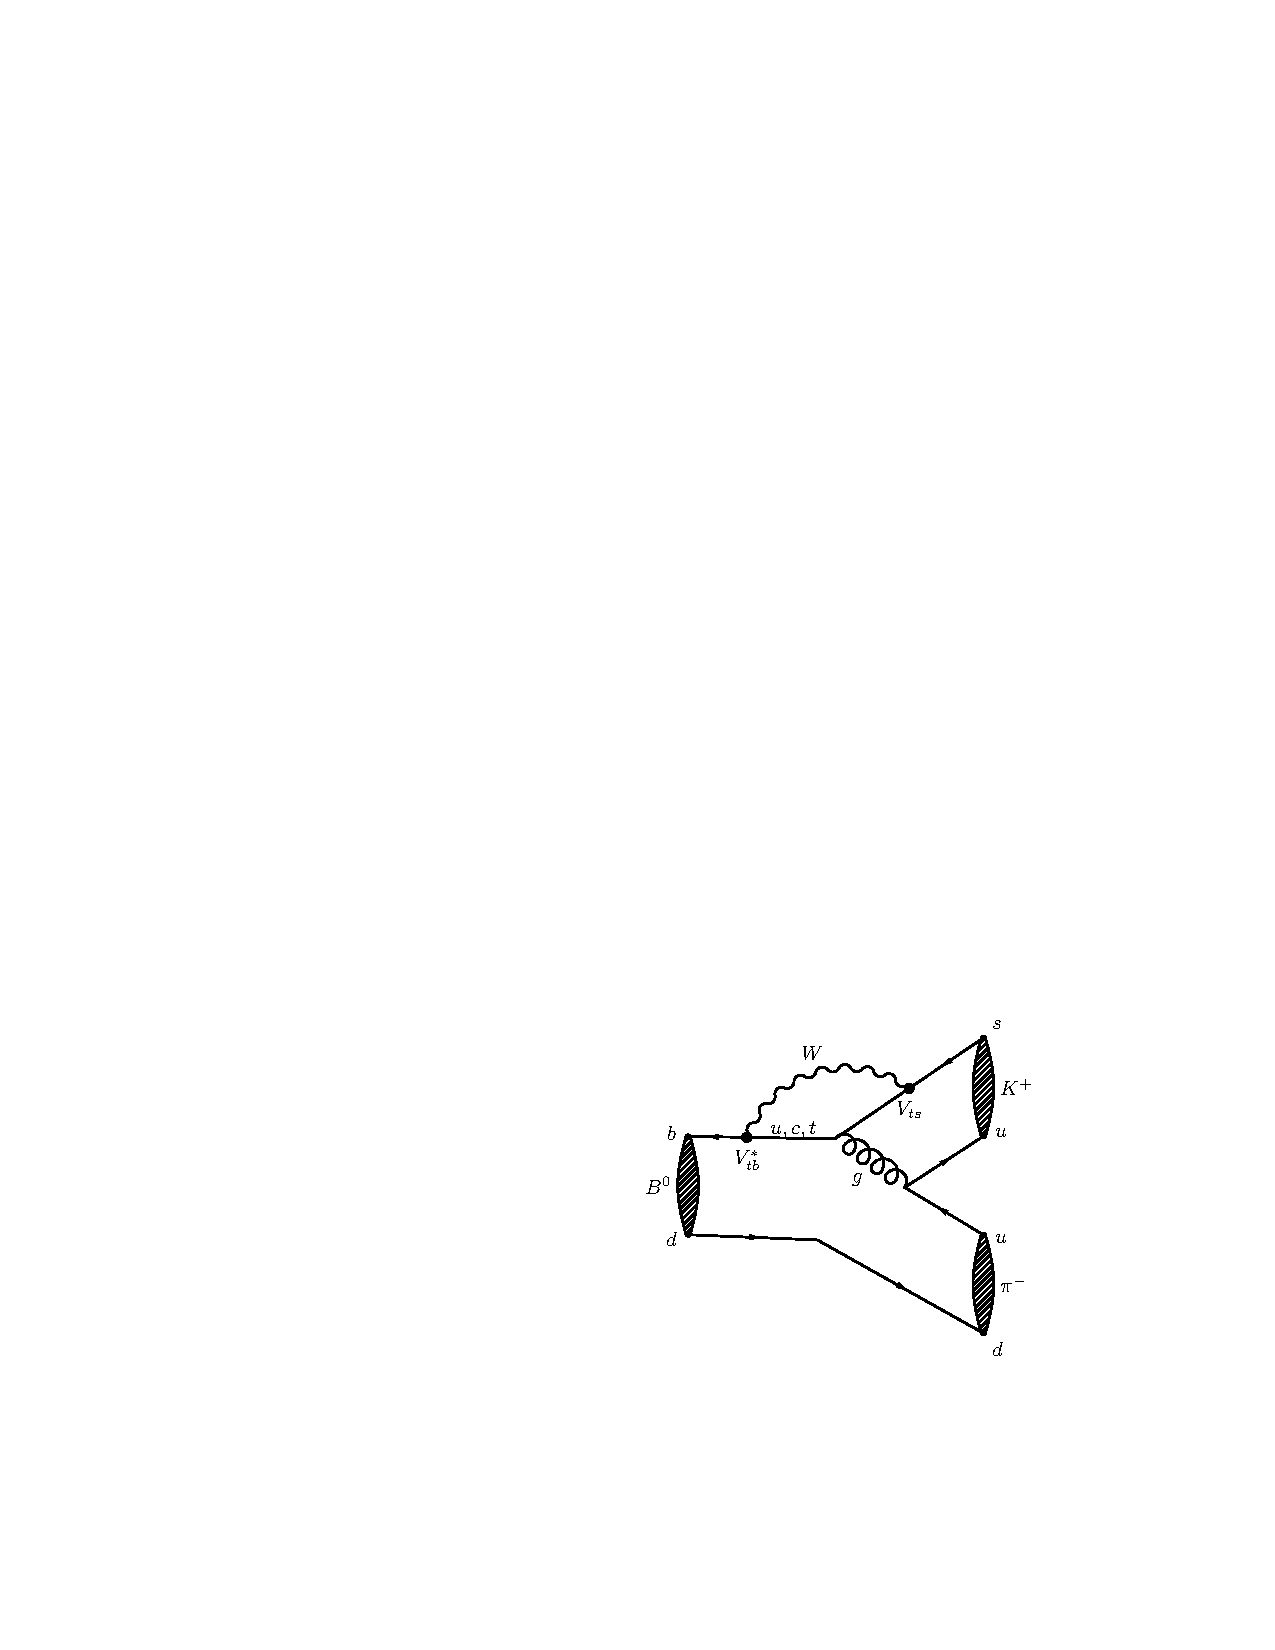
\includegraphics[width=0.4\textwidth]{problemsheets/fig/b_kpi_penguin.pdf}
\end{center}
\item The tree-level diagram has a strong phase $\delta_t$ related to the formation of final state hadrons, which is common for the $B^0$ and $\bar{B}^0$ decays. Similarly the loop-level diagram has a strong phase $\delta_l$. Show that
\[|\mathcal{A}_{B^0}|^2-|\mathcal{A}_{\bar{B}^0}|^2=2a_{t}a_{l}sin(\phi_t-\phi_l)sin(\delta_t-\delta_l)\]
where the magnitude of the tree and loop level amplitudes are $a_t$, $a_l$ respectively and the weak phase of the $B^0$ tree and loop diagrams are written as $\phi_t$ and $\phi_l$ respectively
\end{enumerate}

\NewQuestion{Basic Kinematics and detector design (exam style)}
An experiment is based at an $e^+e^-$ collider with a Centre of Mass energy of 91~GeV. The experiment aims at measuring the rate at which $Z^0$'s decay to a $b$ and a $\bar{b}$ quark.
\begin{enumerate}
\item Draw the Feynman diagram of this process
\item What are the energies and momenta of the out-coming $b$ and $\bar{b}$ quarks?
\item Will the experiment detect the $b$ and $\bar{b}$ quarks directly? If not explain why
\item By assuming that the hadrons containing a $b$ or $\bar{b}$ quark have a proper lifetime of 1~ps and that they carry on average 80\% of the momentum of the $b$ quarks, what is the average distance these hadrons will fly before decaying?
\item Discuss what type of a particle detector component is required in order to make sure experimentalists can separate $Z^0\to b\bar{b}$ decays over $Z^0$ decays to light quarks ($u$,$d$,$s$)
\item What type of detector components are required in order to measure the energies of particles produced from the $Z^0\to b\bar{b}$ process?
\end{enumerate}


%\NewQuestion{Cherenkov Detectors}